\begin{figure}
  \centering
  \begin{subfigure}[t]{0.7\textwidth}
    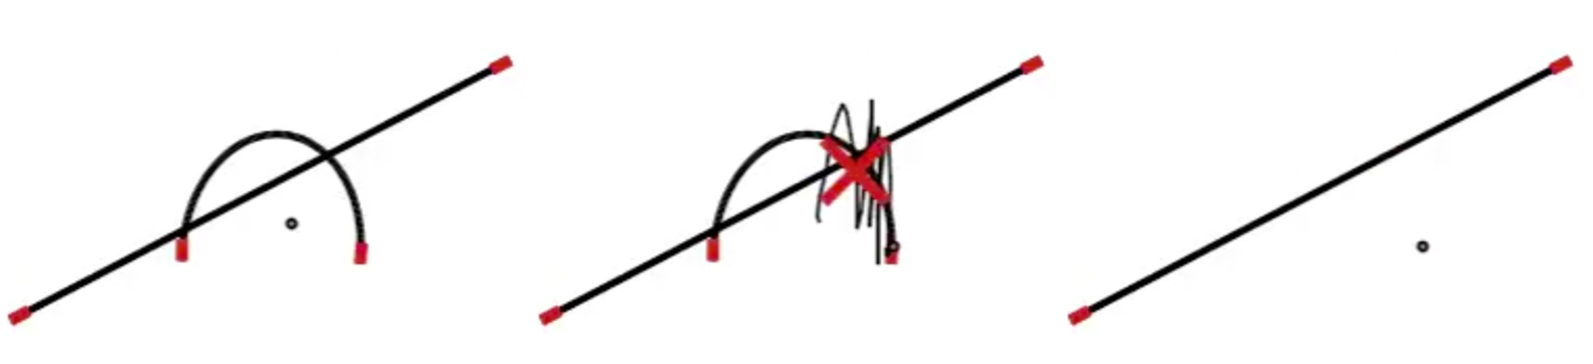
\includegraphics[width=\linewidth]{img/erase-basic.pdf}
    \caption{The erase gesture picks the most specific segments. This
      makes it easy to target short segments that are near or
      overlapping longer ones.}
    \label{fig:erase-basic}
  \end{subfigure}
  \vspace{5mm}

  \begin{subfigure}[t]{0.7\textwidth}
    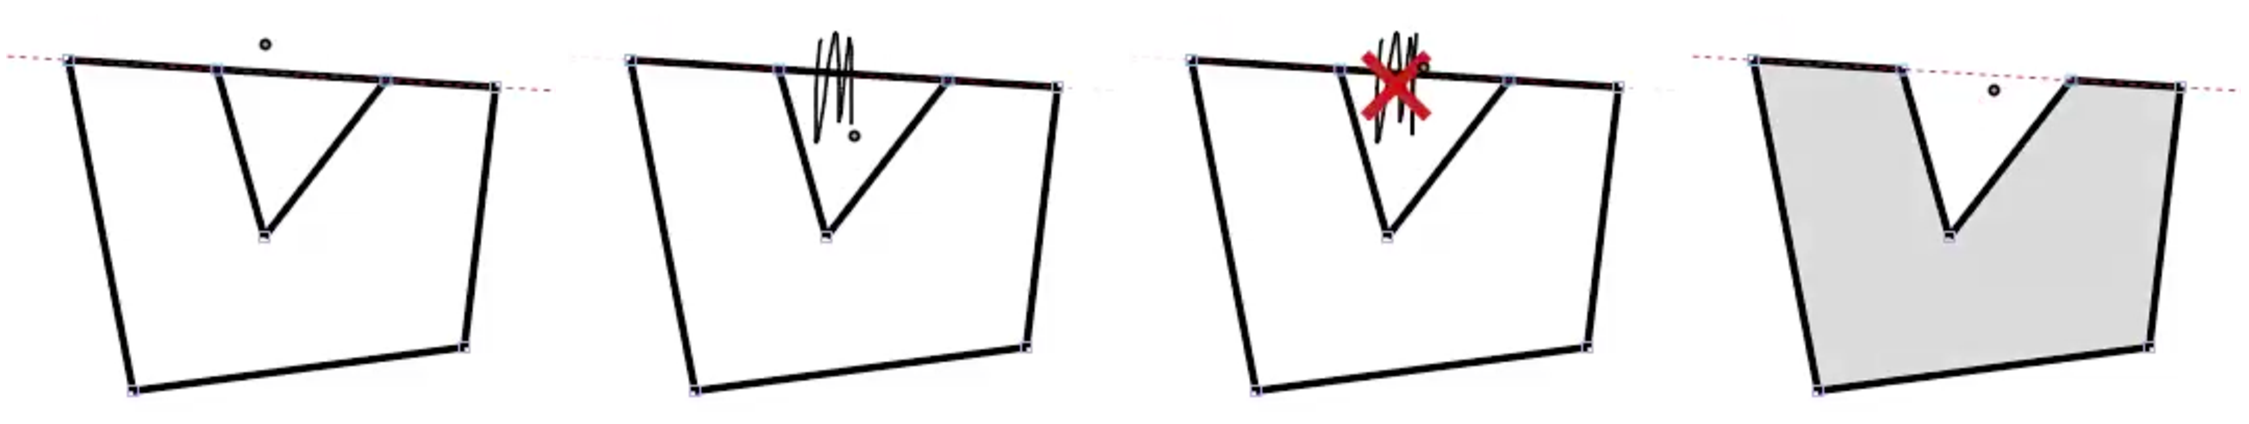
\includegraphics[width=\linewidth]{img/erase-cutout.pdf}
    \caption{Erasing can also be used as part of a deliberate process
      to subtract linework that exposes new shapes.}
    \label{fig:erase-cutout}
  \end{subfigure}
  \caption[Erase gesture]{The erase gesture is made by vigorously
    scribbling. When the dynamic recognizer identifies an erase
    gesture, it gives visual feedback (the red 'X').}
  \label{fig:erase}
\end{figure}
